% Natural Sampling kompakt: Zeitbereich (links) <-> Frequenzbereich (rechts), Zeilen: m, p, m_NS (mit Tiefpass).
% tau/T_s = 0,4 : c_0 = 0,4 ; c_1 = 0,303 ; c_2 = 0,094. Frequenzachse in Einheiten von omega_s, omega_M = 0,32 omega_s.
\begin{center}
\resizebox{.95\linewidth}{!}{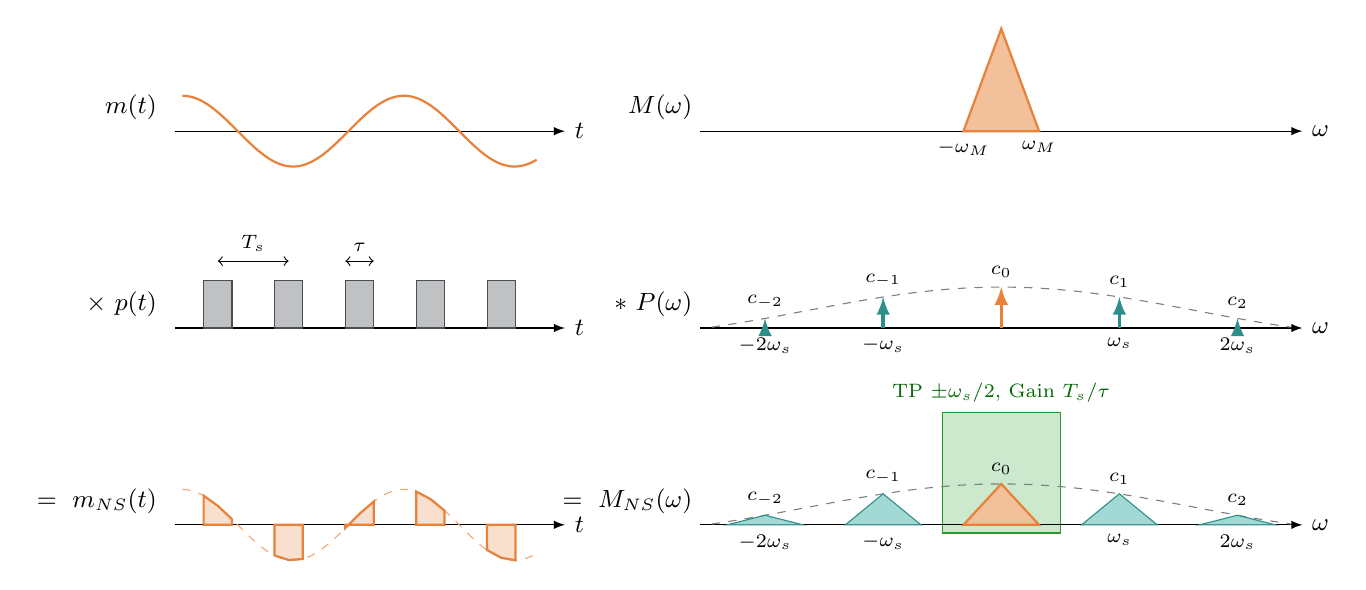
\begin{tikzpicture}[lab/.style={font=\small},tk/.style={font=\scriptsize},ax/.style={-latex,thin}]
\definecolor{org}{HTML}{E8813A}
\definecolor{kA}{HTML}{8CCFCB}\definecolor{kAd}{HTML}{2E8F8A}
\definecolor{ard}{HTML}{4A4D52}
\definecolor{flt}{HTML}{BFE3C0}
\def\pM{0.32}\def\dtau{0.4}
\node[lab,anchor=east] at (1.5,0.3) {$m(t)$};              \node[lab,anchor=east] at (8.3,0.3) {$M(\omega)$};
\node[lab,anchor=east] at (1.5,-2.2) {$\times\ p(t)$};     \node[lab,anchor=east] at (8.3,-2.2) {$\ast\ P(\omega)$};
\node[lab,anchor=east] at (1.5,-4.7) {$=\ m_{NS}(t)$};     \node[lab,anchor=east] at (8.3,-4.7) {$=\ M_{NS}(\omega)$};
% ---------- Zeitbereich ----------
\begin{scope}[shift={(1.7,0)},x=0.9cm,y=1cm]
  \draw[ax] (-0.1,0) -- (5.4,0) node[right,lab] {$t$};
  \draw[org,thick,domain=0:5,samples=50,smooth] plot (\x,{0.45*cos(360*\pM*\x)});
\end{scope}
\begin{scope}[shift={(1.7,-2.5)},x=0.9cm,y=1cm]
  \draw[ax] (-0.1,0) -- (5.4,0) node[right,lab] {$t$};
  \foreach \c in {0.5,1.5,2.5,3.5,4.5} \fill[ard!35,draw=ard] (\c-0.2,0) rectangle (\c+0.2,0.6);
  \draw[<->] (0.5,0.85) -- (1.5,0.85) node[midway,above,tk] {$T_s$};
  \draw[<->] (2.3,0.85) -- (2.7,0.85) node[midway,above,tk] {$\tau$};
\end{scope}
\begin{scope}[shift={(1.7,-5)},x=0.9cm,y=1cm]
  \draw[ax] (-0.1,0) -- (5.4,0) node[right,lab] {$t$};
  \draw[org!70,dashed,domain=0:5,samples=50,smooth] plot (\x,{0.45*cos(360*\pM*\x)});
  \foreach \c in {0.5,1.5,2.5,3.5,4.5}
    \filldraw[fill=org!25,draw=org,thick] (\c-0.2,0) -- plot[domain=\c-0.2:\c+0.2,samples=3] (\x,{0.45*cos(360*\pM*\x)}) -- (\c+0.2,0) -- cycle;
\end{scope}
% ---------- Frequenzbereich (Einheit omega_s, Höhe 1 = Spitze von M) ----------
\begin{scope}[shift={(12.1,0)},x=1.5cm,y=1.3cm]
  \draw[ax] (-2.55,0) -- (2.55,0) node[right,lab] {$\omega$};
  \fill[org!50,draw=org,thick] (-\pM,0) -- (0,1) -- (\pM,0) -- cycle;
  \node[tk,below] at (-\pM,0) {$-\omega_M$}; \node[tk,below] at (\pM,0) {$\omega_M$};
\end{scope}
\begin{scope}[shift={(12.1,-2.5)},x=1.5cm,y=1.3cm]
  \draw[ax] (-2.55,0) -- (2.55,0) node[right,lab] {$\omega$};
  \draw[dashed,gray,domain=-2.45:2.45,samples=50] plot (\x,{\dtau*sin(deg(pi*\dtau*\x))/(pi*\dtau*\x)});
  \foreach \n/\h/\l in {-2/0.094/c_{-2},-1/0.303/c_{-1},1/0.303/c_1,2/0.094/c_2}
    {\draw[-latex,very thick,kAd] (\n,0) -- (\n,\h); \node[tk,above] at (\n,\h) {$\l$};}
  \draw[-latex,very thick,org] (0,0) -- (0,0.4); \node[tk,above] at (0,0.4) {$c_0$};
  \foreach \n/\t in {-2/-2\omega_s,-1/-\omega_s,1/\omega_s,2/2\omega_s} \node[tk,below] at (\n,0) {$\t$};
\end{scope}
\begin{scope}[shift={(12.1,-5)},x=1.5cm,y=1.3cm]
  \fill[flt,opacity=0.8,draw=green!50!black,thin] (-0.5,-0.08) rectangle (0.5,1.1);
  \node[tk,above,text=green!40!black] at (0,1.1) {TP $\pm\omega_s/2$, Gain $T_s/\tau$};
  \draw[ax] (-2.55,0) -- (2.55,0) node[right,lab] {$\omega$};
  \draw[dashed,gray,domain=-2.45:2.45,samples=50] plot (\x,{\dtau*sin(deg(pi*\dtau*\x))/(pi*\dtau*\x)});
  \foreach \n/\h/\l in {-2/0.094/c_{-2},-1/0.303/c_{-1},1/0.303/c_1,2/0.094/c_2}
    {\fill[kA,fill opacity=0.8,draw=kAd] (\n-\pM,0) -- (\n,\h) -- (\n+\pM,0) -- cycle; \node[tk,above] at (\n,\h) {$\l$};}
  \fill[org!50,draw=org,thick] (-\pM,0) -- (0,0.4) -- (\pM,0) -- cycle; \node[tk,above] at (0,0.4) {$c_0$};
  \foreach \n/\t in {-2/-2\omega_s,-1/-\omega_s,1/\omega_s,2/2\omega_s} \node[tk,below] at (\n,0) {$\t$};
\end{scope}
\end{tikzpicture}}
\end{center}
